\section{Problem Definition}
In this section, we first give a formal definition of exact-K recommendation, and then discuss how to transfer it to the Maximal Clique Optimization problem. Finally we provide a baseline approach to tackle the above problem.
%Due to the difference between Exact-K with Top-K recommendation problem,
%we should make a new problem definition formulation and corresponding approach to tackle it.
%In this section,
%we first give an informal description about what is Exact-K recommendation
%and its difference from well-known Top-K recommendation.
%we first give a formal definition and optimization objective for exact-K recommendation,
%and then discuss how to transfer it to Maximal Clique Optimization problem which is a combinatorial optimization problem and is NP-hard.
%Finally we provide a baseline approach to tackle above problem which is called \emph{Naive Node-Weight Estimation Method}.
%\subsection{Exact-K Recommendation}
%In the most traditional scenarios of recommendation system,
%recommended items (like commodities in E-commerce) are shown in a waterfall flow form, that is to say users should scroll the screen and items can be presented one-by-one. 
%Due to the pressure of QPS (Query Per Second) for users interacting with recommendation system server, it is common to return a large amount of ranked items
%(e.g. 50 items in Taobao recommendation system)
%based on CTR (Click-Through-Rate) estimation for example and presented from top to bottom. 
%That is we hope the top ranked items take the most chance to be clicked so that when user scroll the screen and see items top-down,
%the overall click efficiency can be achieved.
%It can be seen as \emph{Top-K} recommendation, because the ranking of items list is important.
%Top-K recommendation problem is well studied for many years in IR research community (refer to some related works in Section \ref{sec:top_k_related}). %\cite{deshpande2004item,cremonesi2010performance,koren2009matrix,rendle2009bpr,wang2017irgan}.
%
%However in many real-world recommendation applications,
%system will return exact $K$ items and show them once all to users.
%That is to say users should not scroll the screen 
%and combination of the $K$ items is shown as a whole \textbf{card}.
%We call it \emph{Exact-K} recommendation problem,
%it's novel and practical,
%the goal of such task is to maximize 
%the chance of clicked or satisfied by a user to the whole card.
%In the most time, various combinations of items in a card may take different chances to be satisfied given a user.
%And meantime items in a card may maintain some constraints between each other to guarantee the user experience of recommendation system
%(e.g. the diversity of categories of the recommended commodities in E-commerce).
%Due to the difference between Exact-K and Top-K recommendation problem,
%we should make a new problem definition formulation and corresponding approach to tackle Exact-K recommendation problem.
\subsection{Exact-K Recommendation}
\label{sec:problem_definition}
Given a set of candidate $N$ items $S=\{s_i\}_{1\le i\le N}$,
our goal is to recommend exact $K$ items $A=\{a_i\}_{1\le i\le K}\subseteq S$ which is shown as a whole card\footnote{Here we suppose that permutation of the $K$ items in a card is not considered in exact-K recommendation.},
so that the combination of items $A$ takes the most chance to be clicked or satisfied by a user $u$.
We denote the probability of $A$ being clicked/satisfied as $P(A,r=1|S,u)$.
Somehow items in $A$ should obey some $M$ constraints between each other as $C=\{c_k(a_i,a_j)=1|a_i\in A,a_j\in A,i\neq j\}_{1\le k\le M}$ or not as $C=\emptyset$, here $c_k$ is a boolean indicator
which will be $1$ if the two items satisfy the constraint.
Overall the problem of exact-K recommendation can be regarded as a (constrained) combinatorial optimization problem,
and is defined formally as follows:
%\vspace{-10pt}
\begin{small}
\begin{eqnarray}
	\label{eq:objective}
	& \max\limits_{A} P(A,r=1|S,u;\theta), \\
	\label{eq:constraints}
	& s.t\ \forall a_i\in A,a_j\in A,i\neq j, \forall c_k\in C, c_{k}(a_i,a_j)=1,
\end{eqnarray}
\end{small}
where $\theta$ is the parameters for function of generating $A$ from $S$ given user $u$, and $r=1$ donates relevance/preference indicator.

In another perspective, we construct a graph $\mathbb{G}(\mathcal{N},\mathcal{E})$ containing $N$ nodes, in which each node $n_i$ in $\mathcal{N}$ represents an item $s_i$ in candidate item set $S$, each edge $e_{ij}$ in $\mathcal{E}$ connecting nodes $(n_i,n_j)$ represents that items $s_i$ and $s_j$ should satisfy the constraints or there is no constraint\footnote{$\mathbb{G}$ is now a complete graph.},
i.e $\forall c_k\in C, c_{k}(s_i,s_j)=1$ or $C=\emptyset$, so it is an undirected graph here.
%You can take Fig. \ref{fig:clique} as an example.
%\yu{The constraint here can be difference of categories, so if two items belong to different categories then there is an edge connecting the corresponding two nodes in graph.}
Intuitively, we can transfer exact-K recommendation into the maximal clique optimization problem. 
That is to say we aim to select a clique\footnote{A clique is a subset of nodes of an undirected graph such that every two distinct nodes in the clique are adjacent; that is, its induced subgraph is complete.}
(i.e characteristics of clique can ensure the constraints defined in Eq. \ref{eq:constraints})
with $K$ nodes from $\mathbb{G}$ where combination of the selected $K$ corresponding items $A$ achieves the maximal objective defined in Eq. \ref{eq:objective}.
You can take Fig. \ref{fig:clique} as an example.
Furthermore, maximal clique problem is proved to be NP-hard \cite{pardalos1994maximum} thus it can not be solved in polynomial time.
\begin{figure}[th]
	%\vspace{-10pt}
	\centering
	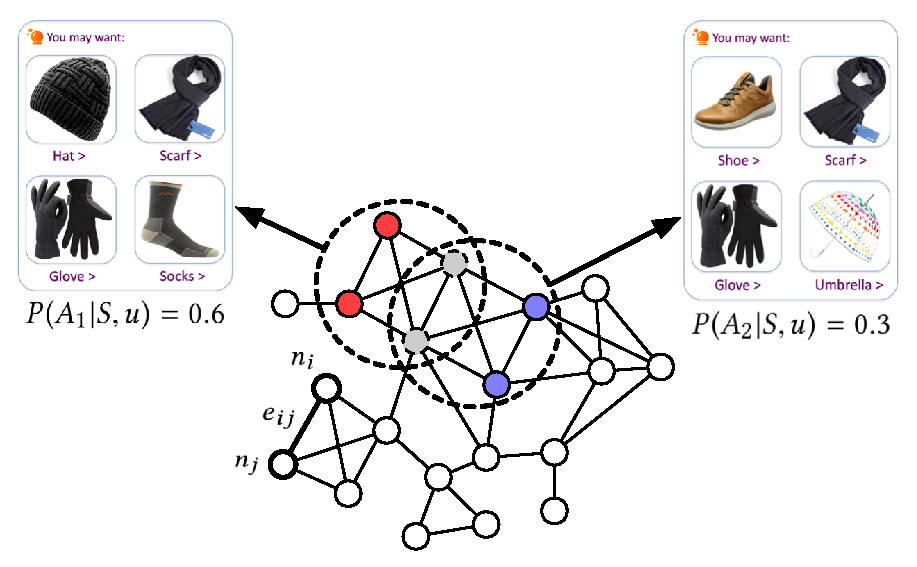
\epsfig{file=figures/clique.eps, width=0.73\columnwidth}
	%\vspace{-10pt}
	\caption{Illustration for a specific graph $\mathbb{G}$ with $N=20$ and $K=4$.
	We show two different cliques (red and blue) in graph and the corresponding cards ($A_1$ and $A_2$) each with 4 items.
	We suppose that $P(A_1|S,u)>P(A_2|S,u)$ means that card $A_1$ takes more chance to be satisfied than card $A_2$ given user $u$ and candidate item set $S$.}
	\label{fig:clique}
	%\vspace{-10pt}
\end{figure}

\subsection{Naive Node-Weight Estimation Method}
\label{sec:nnwem}
A baseline method is that we can estimate a weight as $w_i$ of each node $n_i\in \mathcal{N}$ related to the optimization objective in graph $\mathbb{G}$.
In exact-K recommendation, our goal is to maximize the clicked or satisfied probability of the recommended $K$ items set as in Eq. \ref{eq:objective},
so we regard the weight of each node as CTR of corresponding item.
After getting the weight of each node in graph supported as $\mathbb{G}(\mathcal{N},\mathcal{E},\mathcal{W})$,
we can reduce the Maximal Clique Optimization problem as  
finding a clique in graph $\mathbb{G}$ with maximal node weights summation.
We can then apply some heuristic methods like Greedy search to solve it.
Specifically, we modify Eq. \ref{eq:objective} as follows:
%You can refer to Algorithm \ref{alg:naive} for details\footnote{In our problem, we ignore the circumstance of getting infeasible solution, and we argue that in real-world
%application with small $K$ and large $N$ we can always find a clique with $K$ nodes in graph with $N$ nodes greedily.}.
%The objective function of corresponding reduced problem (here we omit the constraint function as it is the same with Equation \ref{eq:constraints} can be defined as follows:
%\vspace{-10pt}
\begin{small}
\begin{equation}
	\max\limits_{A} \sum_{a_i\in A}{P(r=1|a_i,S,u;\theta)},
\end{equation}
\end{small}
where $P(r=1|a_i,S,u;\theta)$ can be regarded as node weight $w_i$ in graph.
Here we focus on how to estimate the node weights $\mathcal{W}$,
it can be formulated as a normal item CTR estimation task in IR.
%and large amount of Learning to Rank based methods are proposed.
%Some more details are described in Sec. \ref{sec:ltr} 
%which can be adopted as our strong baselines.
A large amount of LTR based methods for CTR estimation can be adopted as our strong baselines. Refer to Sec. \ref{sec:ltr} for more details. 
%\begin{algorithm}
%	\caption{Naive Node-Weight Estimation Method.}       
%	\label{alg:naive} 
%	\begin{algorithmic}[1]
%		\Require Given user $u$ and candidate items set $S$, construct graph $\mathbb{G}(\mathcal{N},\mathcal{E})$ defined in paragraph 2 of Section \ref{sec:problem_definition}.
%		\State Estimate weight $w_i$ of each node $n_i\in \mathcal{N}$ in graph based on CTR of corresponding item $s_i\in S$.
%		\State Initial result card $A=\emptyset$.
%		\For {\emph{t = 1 to K}}
%		\State Select node $a_t$ with the largest weight in $\mathcal{N}$ and add to $A$.
%		\State Remove $a_t$ and nodes in $\mathcal{N}$ which are not adjacent to $a_t$.
%		\EndFor\\
%		\Return result card $A$.
%	\end{algorithmic}
%\end{algorithm}

%We call our above discussed baseline approach as Naive Node-Weight Estimation Method
%(refer to Algorithm \ref{alg:naive} for details
We call the adapted baseline as Naive Node-Weight Estimation Method, with its detailed implementation shown in Algorithm \ref{alg:naive}~\footnote{In our problem, we ignore the circumstance of getting infeasible solution, and we argue that in real-world application with small $K$ and large $N$ we can always find a clique with $K$ nodes in graph with $N$ nodes greedily.}.
However weaknesses of such method are obvious for the following three points:
\begin{inparaenum}
\item CTR estimation for each item is independent, 
\item combinational characteristic of the $K$ items in a card is not considered,
\item problem objective is not optimized directly but substituted with a reduced heuristic objective which will unfortunately fall into sub-optimal.
\end{inparaenum}
On the contrary, we will utilize a framework of Neural Combinatorial Optimization (some related works in Sec. \ref{sec:nco_related}) to directly optimize the problem objective in Sec. \ref{sec:approach}.
%\begin{algorithm}
%	\caption{Naive Node-Weight Estimation Method.}       
%	\label{alg:naive} 
%	\begin{algorithmic}[1]
%		\STATE Given user $u$ and candidate items set $S$, construct graph $\mathbb{G}(\mathcal{N},\mathcal{E})$ defined in paragraph 2 of Section \ref{sec:problem_definition}.
%		\STATE Estimate weight $w_i$ of each node $n_i\in \mathcal{N}$ in graph based on CTR of corresponding item $s_i\in S$.
%		\STATE Rank $\mathcal{N}$ based on node weight as $Q$.
%		\REPEAT
%		\STATE Initial result card $A=\emptyset$.
%		\STATE Copy graph $\mathbb{G}(\mathcal{N},\mathcal{E})$ as $\mathbb{G'}(\mathcal{N'},\mathcal{E'})$.
%		\FOR {\emph{t = 1 to K}}
%		\IF{$t = 1$}
%		\STATE Select the top node of $Q$ and add to $A$.
%		\ELSE 
%		\STATE Select node with the largest weight in $\mathcal{N'}$ and add to $A$.
%		\ENDIF
%		\STATE Remove all nodes in $\mathcal{N'}$ which are not adjasen to any of node in $A$ (including $A$).
%		\ENDFOR
%		\IF{$|A|\neq K$}
%		\STATE Pop the top node in $Q$.
%		\ENDIF
%		\UNTIL{$|A|=K$.}
%		\STATE return result card $A$.
%	\end{algorithmic}
%\end{algorithm}

